\chapter{SoC Block Design}

\section{Task Description}

The BASYS3 dice project uses a Vivado block design called \texttt{soc\_top}
for the processor subsystem. The subsystem provides memory, serial I/O,
GPIO, timing, and access to the external display and LED controllers.

\section{Block Design}

The archived design uses the MicroBlaze 11.0 IP with 128\,KiB of local block
RAM. The AXI crossbar connects the processor to GPIO, UART Lite, a timer,
an interrupt controller, and the peripheral bridges. The address map of the
integrated design is listed in Table~\ref{tab:address-map}.

\IfFileExists{figures/final/block-design.png}{%
  \evidencefigure{block-design.png}{Vivado block design used for the final board build.}{fig:final-bd}{}
}{%
  \todo{Add a readable Vivado export of the final block design.}
  \begin{figure}[!ht]
    \centering
    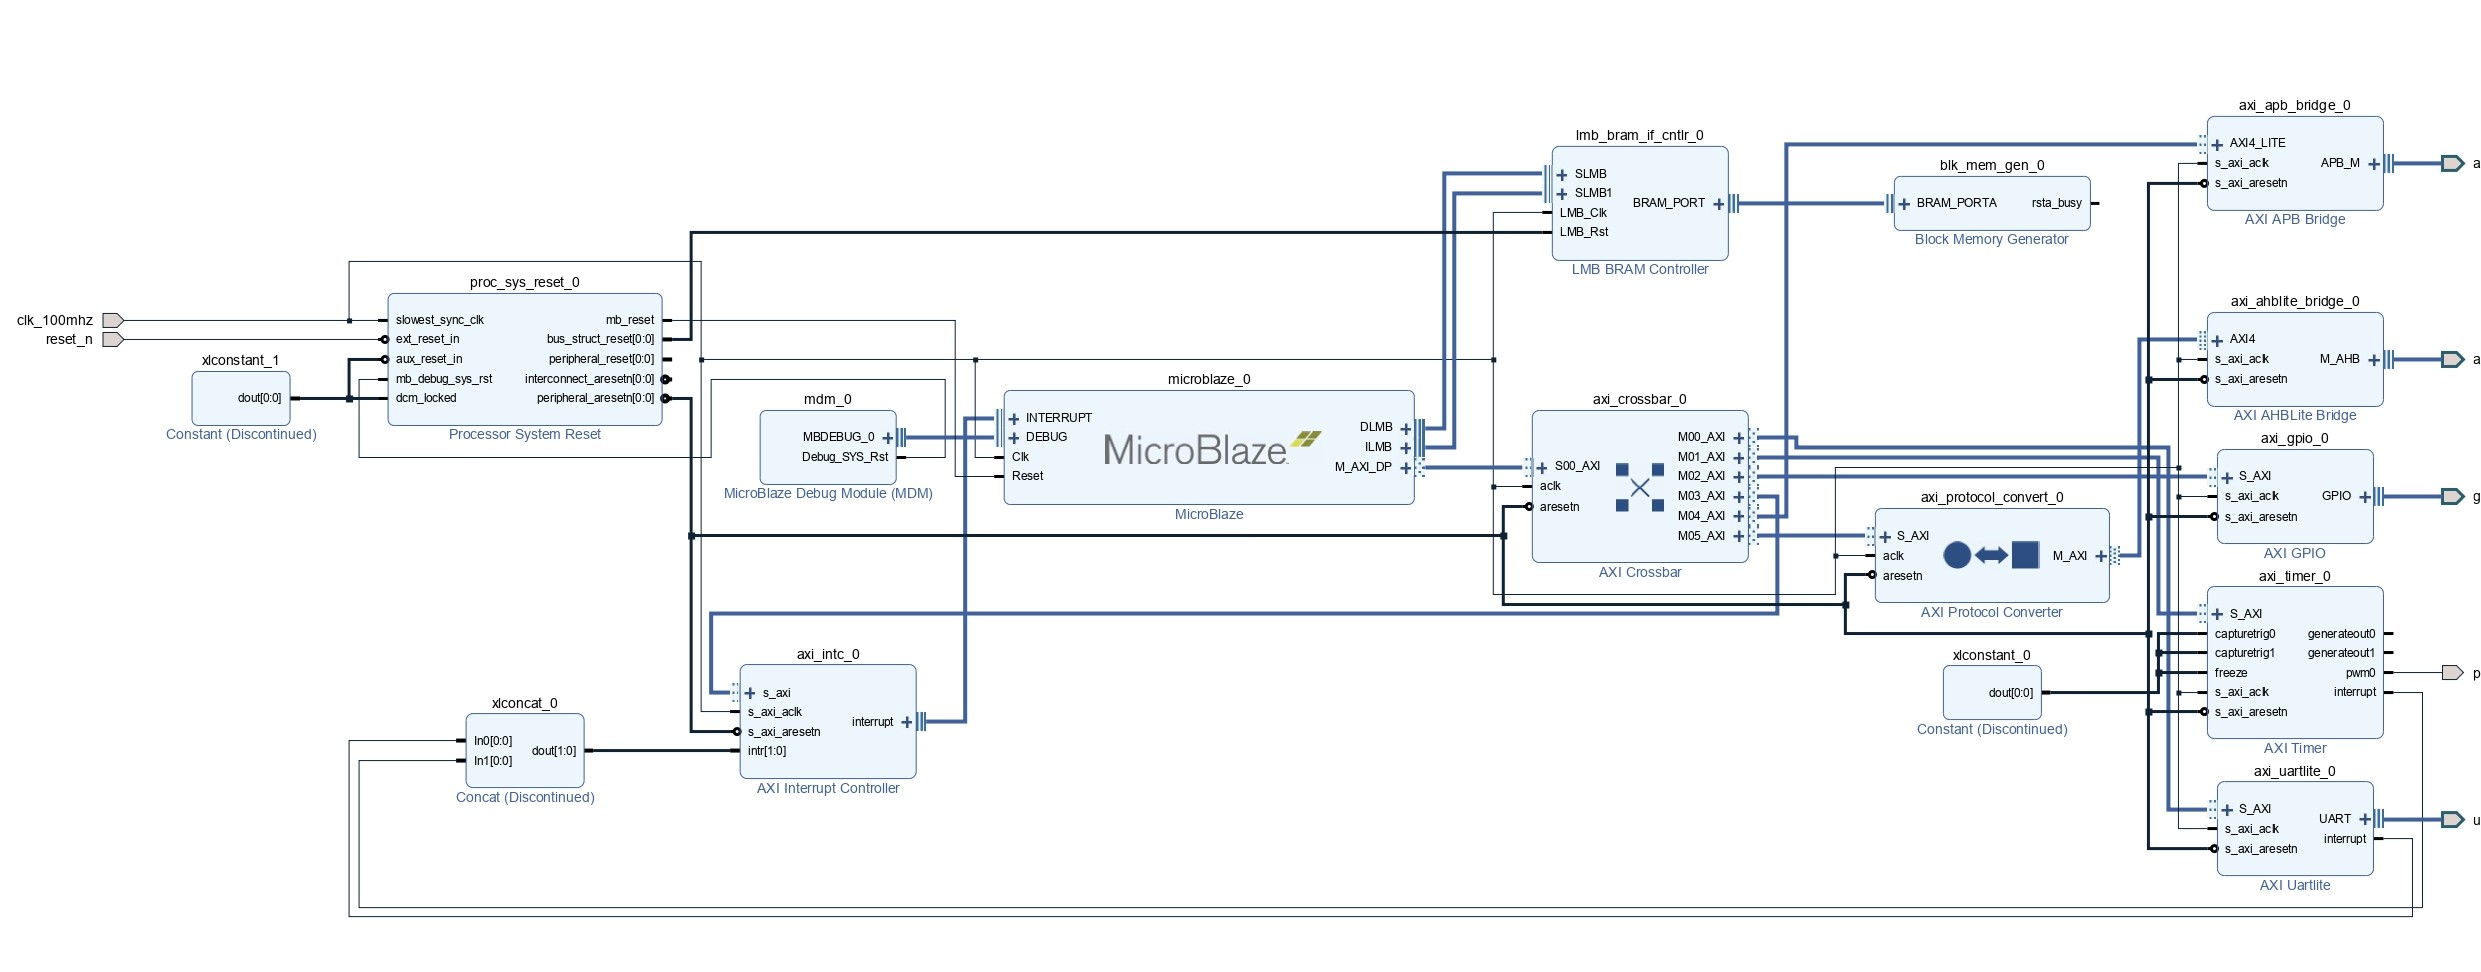
\includegraphics[width=\linewidth]{figures/Lab1/BlockDesign.jpg}
    \caption{Earlier Vivado block design with the APB and AHB-Lite bridges.}
    \label{fig:earlier-bd}
  \end{figure}%
}
